\section{Template Matching}

\subsection{Überlegungen}
Jetzt wo ich die Kreiserkennung implementiert habe, ist es mir möglich Münzen im Bild zu erkennen. Der nächste Schritt wäre es nun, die Münzen zu klassifizieren und zu unterscheiden. Doch wie klassifiziert man in openCV Bilder? Eine Möglichkeit ist das Template Matching. Dabei wird ein Template, also eine Vorlage, über ein Bild geschoben und die Ähnlichkeit an jedem Punkt beziehungsweise Pixel berechnet. Das Ergebnis ist eine Heatmap, die die Übereinstimmung an jedem Punkt im Bild anzeigt.

\subsection{Die Vorlagen}
Damit ich die Münzen anhand ihrer Bildinformastionen klassifizieren kann, benötige ich zuerst Vorlagen, mit denen ich die Münzen vergleichen kann. Ich habe also Bilder von den Münzen gemacht und diese als Vorlagen gespeichert. Diese Vorlagenbilder sind die Referenzbilder, anhand derer ich die Münzen im Kamerabild auf Ähnlichkeit überprüfen möchte.

Hier hat sich vorallem die spiegelnde Oberfläche der Münzen als Problem herausgestellt. Ich musste viel mit dem Lichteinfallswinkel und der Beleuchtung spielen, um von jeder Münze ein gutes Bild zu bekommen. Auch der Abnutzungsgrad hat das Erstellen der Vorlagen erschwert. So musste ich vorallem bei den 50-20-10 Cent Münzen und bei den 5-2-1 Cent Münzen darauf achten, dass die Münzen stets eine ähnliche Optik ausweisen. Andernfalls könnte es passieren, dass die Spiegelung oder die Abnutzung als Unterschied interpretiert wird und nicht mehr die Ziffern auf den Münzen.

Meine Vorlagen sehen wie folgt aus:

\begin{figure}[ht]
    \centering
    \begin{subfigure}{0.23\textwidth}
        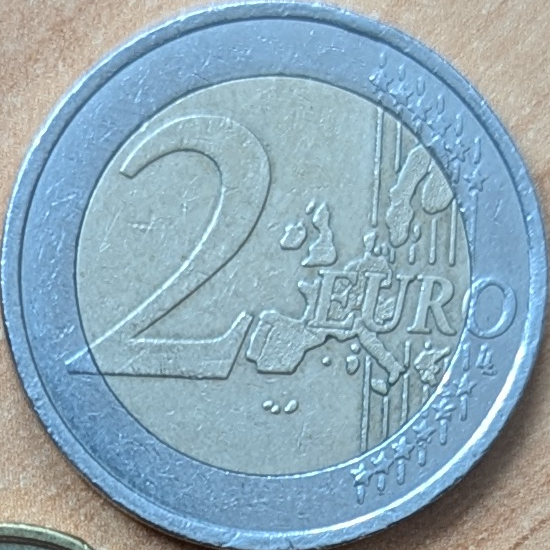
\includegraphics[width=\linewidth]{../CoinFinder/templates_2/Euro2.png}
    \end{subfigure}
    \begin{subfigure}{0.23\textwidth}
        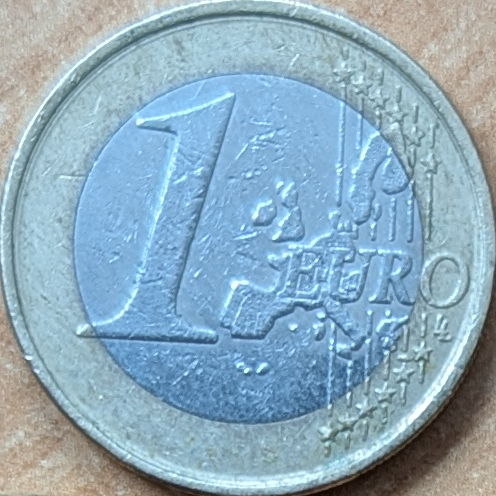
\includegraphics[width=\linewidth]{../CoinFinder/templates_2/Euro1.png}
    \end{subfigure}
    \begin{subfigure}{0.23\textwidth}
        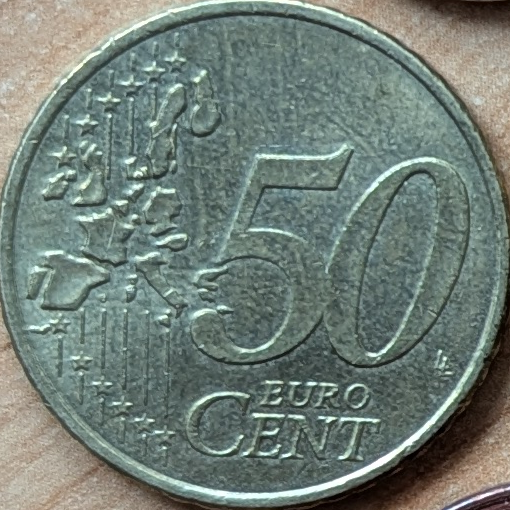
\includegraphics[width=\linewidth]{../CoinFinder/templates_2/Cent50.png}
    \end{subfigure}
    \begin{subfigure}{0.23\textwidth}
        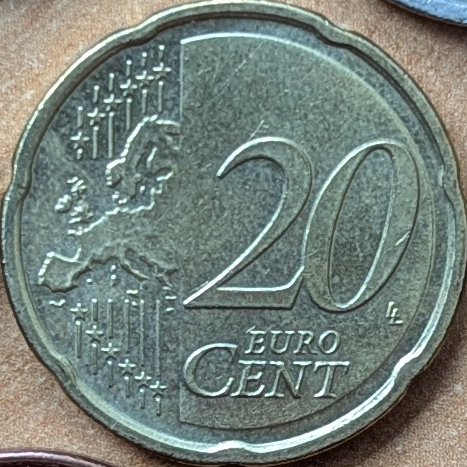
\includegraphics[width=\linewidth]{../CoinFinder/templates_2/Cent20.png}
    \end{subfigure}

    \begin{subfigure}{0.23\textwidth}
        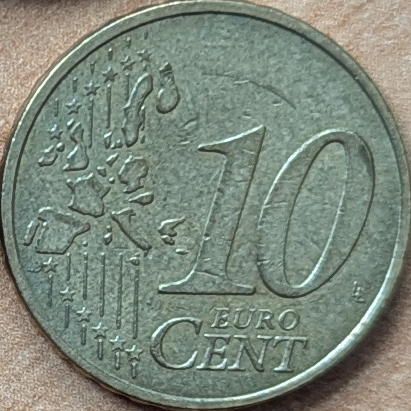
\includegraphics[width=\linewidth]{../CoinFinder/templates_2/Cent10.png}
    \end{subfigure}
    \begin{subfigure}{0.23\textwidth}
        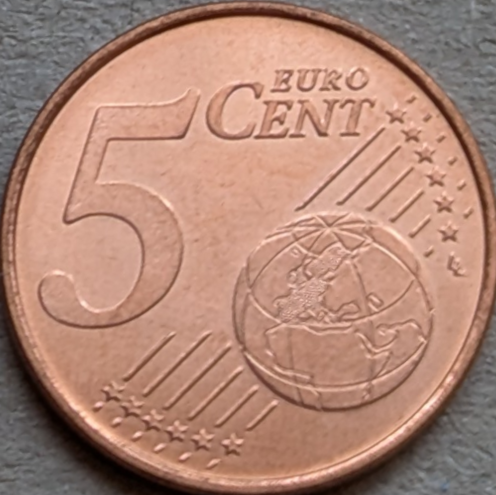
\includegraphics[width=\linewidth]{../CoinFinder/templates_2/Cent5.png}
    \end{subfigure}
    \begin{subfigure}{0.23\textwidth}
        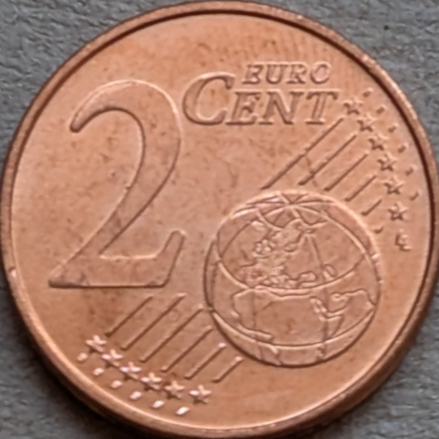
\includegraphics[width=\linewidth]{../CoinFinder/templates_2/Cent2.png}
    \end{subfigure}
    \begin{subfigure}{0.23\textwidth}
        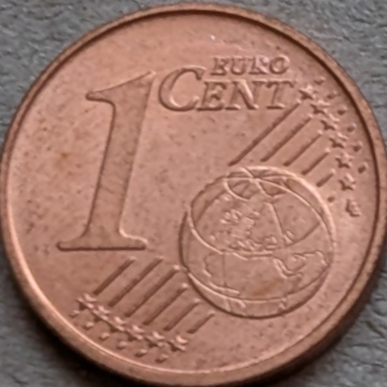
\includegraphics[width=\linewidth]{../CoinFinder/templates_2/Cent1.png}
    \end{subfigure}
\end{figure}

Bevor ich nun mit dem Vergleich der Vorlagen beginne, brauche ich zunächst eine Möglichkeit um sowohl die Vorlagen als auch die daraus resultierenden Ergebnisse zu speichern. Dafür habe ich ein global verfügbares Objekt \textit{COINS} erstellt, welches die Münzen als Schlüssel enthält und als Wert ein Objekt mit den Eigenschaften \textit{diameter} und \textit{value} hat. Weitere Eigenschaften können dann zur Laufzeit den einzelnen Münzen hinzugefügt werden.

\begin{lstlisting}[style=JavaScript]
let COINS = {
    Euro2 : {
        diameter: 25.75,
        value: 2
    },
    Euro1 : {
        diameter: 23.25,
        value: 1
    },
    Cent50 : {
        diameter: 24.25,
        value: 0.5
    },
    Cent20 : {
        diameter: 22.25,
        value: 0.2
    },
    Cent10 : {
        diameter: 19.75,
        value: 0.1
    },
    Cent5 : {
        diameter: 21.25,
        value: 0.05
    },
    Cent2 : {
        diameter: 18.75,
        value: 0.02
    },
    Cent1 : {
        diameter: 16.25,
        value: 0.01
    }
}    
\end{lstlisting}

Diese Datenstruktur kann ich nun verwenden, um die Vorlagen zu speichern und ihnen eine Münze zuzuordnen. In der folgenden Methode iteriere ich über jede Münze und lese das Vorlagenbild ein:

\begin{lstlisting}[style=JavaScript]
const templatesLoaded = new Event('templatesLoaded');
let path = "../Templates/"

function InitTemplates() {
    let coinLength = Object.keys(COINS).length;
    let loadedCoins = 0;
    Object.entries(COINS).forEach(([key, value]) => {
        //is in the template folder a picture with the same name as the key?
        let img = new Image();

        img.onload = () => {
            //save image as matrix in the coin object
            COINS[key].template = cv.imread(img);

            loadedCoins++;
            if(loadedCoins === coinLength){
                document.dispatchEvent(templatesLoaded);
            }
        }

        img.onerror = () => {
            console.log("error: " + key);
        }

        img.src = path + key + ".png";

    });
}
\end{lstlisting}

Das Event \textit{templatesLoaded} wird ausgelöst, sobald alle Vorlagen geladen wurden. Somit kann ich sicherstellen, dass Programmschritt welche die Vorlagen benötigen erst ausgeführt werden, wenn die Vorlagen auch wirklich geladen wurden.
\subsection{Funktionsweise}
Template Matching funktioniert in openCV.js mit der folgenden Funktion:
\begin{lstlisting}[style=JavaScript]
cv.matchTemplate(image, templ, result, method, mask);
\end{lstlisting}

Lasst uns die Parameter genauer betrachten:
\begin{itemize}
    \item \textbf{image} - Das Bild, in dem das Template gesucht werden soll. Es muss als openCV-Matrix vorliegen.
    \item \textbf{templ} - Das Template, das gesucht werden soll. Es muss auch als openCV-Matrix vorliegen.
    \item \textbf{result} - Die Heatmap, in der die Übereinstimmung an jedem Punkt im Bild gespeichert wird. Auch diese muss als openCV-Matrix vorliegen.
    \item \textbf{method} - Die Methode, die zur Berechnung der Übereinstimmung verwendet werden soll. Aktuell gibt es folgende Methoden in openCV.js:
    \subitem \textbf{cv.TM\_SQDIFF} - Summe der quadrierten Differenzen (kleinere Werte bedeuten bessere Übereinstimmung)
    \subitem \textbf{cv.TM\_SQDIFF\_NORMED} - Normalisierte Summe der quadrierten Differenzen (kleinere Werte bedeuten bessere Übereinstimmung)
    \subitem \textbf{cv.TM\_CCORR} - Kreuzkorrelation (größere Werte bedeuten bessere Übereinstimmung)
    \subitem \textbf{cv.TM\_CCORR\_NORMED} - Normalisierte Kreuzkorrelation (größere Werte bedeuten bessere Übereinstimmung)
    \subitem \textbf{cv.TM\_CCOEFF} - Kreuzkorrelationskoeffizient (größere Werte bedeuten bessere Übereinstimmung)
    \subitem \textbf{cv.TM\_CCOEFF\_NORMED} - Normalisierter Kreuzkorrelationskoeffizient (größere Werte bedeuten bessere Übereinstimmung)
    \item \textbf{mask} - (optional) Eine Maske, die angibt, welche Bereiche des Bildes berücksichtigt werden sollen. In meinem Fall benutze ich keine Maske, da ich bereits vor Aufruf der Funktion unwerwünschte Bereiche des Bildes ausschneide.
\end{itemize}

Meine Funktion für das Template Matching sieht nun so aus:
\begin{lstlisting}[style=JavaScript]
function MatchTemplates(src, circle){
    //create result string
    let resultsString = [];
    Object.entries(COINS).forEach(([key, value]) => {
        let resultMat = new cv.Mat();

        //resize template to the size of src
        let templateResized = new cv.Mat();
        cv.resize(COINS[key].template, templateResized, COINS[key].template.size(), 0, 0, cv.INTER_AREA);

        cv.matchTemplate(src, templateResized, resultMat, cv.TM_SQDIFF_NORMED);

        //get highest value
        let minMax = cv.minMaxLoc(resultMat);
        let min = minMax.minVal;

        resultsString.push(new Result(key, min));

        templateResized.delete();
    });

    //sort results from highest to lowest
    resultsString.sort((a, b) => a.value - b.value);

    //console.dir(resultsString);

    //save bestmatch in circle
    circle.bestMatch = COINS[resultsString[0].name];
    circle.matchValue = resultsString[0].value;

    //set matchValue to 2 decimal places
    circle.matchValue = Math.round(circle.matchValue * 100) / 100;

    src.delete();
}
\end{lstlisting}

Innerhalb des main-loops wird diese Funktion nun für jeden gefundenen Kreis ausfgerufen. Der Parameter "src" ist dabei eine ausgeschnittene Region des Bildes, in der sich der Kreis befindet. Der Parameter "circle" ist das Circle-Objekt, in dem die Informationen zum Kreis gespeichert sind. Die Funktion iteriert anschließend über alle Vorlagen und berechnet die Übereinstimmung für jede Vorlage. Hierbei muss beachtet werden, dass Vorlage und das zu prüfende Bild vorher auf die selbe Größe gebracht werden müssen. Die Ergebnisse werden in einem Array gespeichert und anschließend sortiert. Das beste Ergebnis wird dann im Circle-Objekt gespeichert.

\subsection{Exkurs: Mehrere Matrizen in einem Canvas anzeigen}
Bei wachsender Komplexität der Webanwendung ob ich mir immer wieder gewünscht eine Möglichkeit zu haben, mehrere Matrizen in einem Canvas anzuzeigen. Dies ist standardmäßig in openCV.js nicht vorgesehen, da die Funktion \textit{cv.imshow()} immer nur eine Matrix anzeigen kann. Also habe ich mir eine eigene Funktion geschrieben, die mehrere Matrizen in einem Canvas anzeigen kann. Diese Funktion sieht so aus:

\begin{lstlisting}[style=JavaScript]
function ShowMatrices(src, canvas) {
    if (src.length === 0) {
        console.error("No src to show");
        return;
    }

    if (src.length === 1) {
        console.warn("Only one matrix to show. Using ShowMatrix instead");
        ShowMatrix(src[0], canvas);
        return;
    }

    let numberOfMatrices = src.length;

    // Berechnung der Gittergröße
    let gridCols = Math.ceil(Math.sqrt(numberOfMatrices));
    let gridRows = Math.ceil(numberOfMatrices / gridCols);

    // Maximalbreite und -höhe der Matrizen basierend auf der Größe des Canvas
    let cellWidth = canvas.width / gridCols;
    let cellHeight = canvas.height / gridRows;

    // Canvas leeren
    let ctx = canvas.getContext('2d');
    ctx.clearRect(0, 0, canvas.width, canvas.height);

    // Jede Matrix im Gitter zeichnen
    src.forEach((mat, index) => {
        // Spalte und Zeile bestimmen
        let col = index % gridCols;
        let row = Math.floor(index / gridCols);

        // Zielbereich für diese Matrix
        let x = col * cellWidth;
        let y = row * cellHeight;
        let targetSize = new cv.Size(cellWidth, cellHeight);

        // Matrix auf passende Größe skalieren
        let resizedMat = new cv.Mat();
        cv.resize(mat, resizedMat, targetSize, 0, 0, cv.INTER_AREA);

        // Matrix in RGBA umwandeln wenn es sich um eine Graustufenmatrix handelt
        if (resizedMat.channels() === 1) {
            let rgbaMat = new cv.Mat();
            cv.cvtColor(resizedMat, rgbaMat, cv.COLOR_GRAY2RGBA);
            resizedMat.delete();
            resizedMat = rgbaMat;
        }

        // Erstelle ein temporäres Canvas für diese Matrix
        let tempCanvas = document.createElement('canvas');
        let tempCtx = tempCanvas.getContext('2d');
        tempCanvas.width = resizedMat.cols;
        tempCanvas.height = resizedMat.rows;

        // In ein ImageData konvertieren und in das temporäre Canvas zeichnen
        let imageData = new ImageData(new Uint8ClampedArray(resizedMat.data), resizedMat.cols, resizedMat.rows);
        tempCtx.putImageData(imageData, 0, 0);

        // Zeichne das temporäre Canvas auf das Haupt-Canvas
        ctx.drawImage(tempCanvas, 0, 0, resizedMat.cols, resizedMat.rows, x, y, cellWidth, cellHeight);

        // Bereinige die temporären Matrizen
        resizedMat.delete();
    });
}
\end{lstlisting}

Um mehrere Bilder in einen Canvas zu zeichnen, musste ich die Größe der Bilder anpassen, damit sie in ein Grid passen. Dafür habe ich die Funktion \textit{cv.resize()} verwendet. Anschließend müssen die Matrizen zuerst in ein temporäres Canvas gezeichnet werden, bevor sie in das Haupt-Canvas gezeichnet werden können. Die Funktion \textit{drawImage()} von Canvas kann nur Bilder zeichnen, keine Matrizen. Daher musste ich die Matrizen in ein ImageData-Objekt umwandeln, bevor ich sie in das Canvas zeichnen konnte.
\subsection{Erste Ergebnisse}
Es hat sich gezeigt, dass der Vergleich der Vorlagen prinzipiell funktionieren kann. Jedoch ist die Genauigkeit  noch nicht zufriedenstellend. Münzen können zwar grob in die richtige Kategorie eingeordnet werden (sprich 1-2-5 Cent Münzen und 10-20-50 Cent Münzen), jedoch ist die Unterscheidung innerhalb dieser Kategorien nicht funktional. So werden aktuell nur maximal die Hälfte der Münzen korrekt zugeordnet.

Es scheint, als wären die Informationen der Ziffern auf den Münzen nicht ausreichend, um eine genaue Klassifizierung zu ermöglichen. Die Farbe einer Münze hat im Gegensatz dazu einen relativ großen Einfluss auf das Ergebnis. So werden Münzen meist der korrekten Farbkategorie zugeordnet, jedoch nicht derm korrekten Wert. Dies ist ein Hinweis darauf, dass die Farbinformationen der Münzen stärker gewichtet werden als die Forminformationen. Da sich Münzen innerhalb einer Kategorie (z.B. 1-2-5 Cent Münzen) jedoch nur in der Größe und ihrer Ziffer optisch unterscheiden, ist es schwierig eine weitere Methode der Klassifizierung zu finden. Ein Prüfen der Größe würde in meinem Anwendungsfall nicht funktionieren, da sowohl der Abstand zur Kamera als auch die Position der Münzen im Bild variabel sind. 

Eine Möglichkeit die Genauigkeit zu erhöhen wäre es, den störenden Faktor der Farbinformationen zu eliminieren, und stattdessen nur Vorlagen zu verwenden, welche nur die notwendigen Informationen enthalten. Dies könnte z.B. durch das Erstellen von Kantenbildern der Münzen erreicht werden. Solche Bilder wie sie vom Canny-Algorithmus erstellt werden, enthalten nur die Kanten des Ausgangsbildes und keine Farbinformationen, da sie rein als Schwarz-Weiß-Bilder vorliegen. Diese Kantenbilder könnten dann an Stelle der aktuellen Farbbilder als Vorlagen verwendet werden.

Jedoch gibt es noch ein weiteres Problem: die Rotation. Bereits eine kleine Drehung des Ausgangsbildes verursacht große Unterschiede in der Übereinstimmung. Das Template Matching in openCV berechnet standardmäßig nur die Übereinstimmung für das Template in der gleichen Rotation wie das Bild. Dies ist ein Problem, da die Münzen im Kamerabild in unterschiedlichen Rotationen vorkommen können. Eine Möglichkeit dieses Problem zu lösen wäre es, das Template in verschiedenen Rotationen zu speichern und für jede Rotation die Übereinstimmung zu berechnen. Dies würde jedoch die Anzahl der Vorlagen vervielfachen und einen unverhältnismäßig hohen Aufwand bedeuten. Eine andere Möglichkeit wäre es, das Ausgangsbild mehrfach zu rotieren und für jede Rotation die Übereinstimmung zu den Vorlagen berechnen. So wäre bei ausreichend kleingranularer Rotation sichergestellt, dass jede Münze mindestens einmal eine ähnliche Ausrichtung wie das zutreffende Template hat. Dies würde jedoch die Rechenzeit signifikant erhöhen, da bedeutend mehr Berechnungen pro Münze durchgeführt werden müssten. Zudem braucht es dafür eine Möglichkeit, alle Zwischenergebnisse der Rotationen zu speichern, um anschließend das beste Ergebnis zu wählen.